%This work is licensed under the Creative Commons Attribution-NonCommercial-NoDerivs 3.0 United States License. To view a copy of this license, visit http://creativecommons.org/licenses/by-nc-nd/3.0/us/ or send a letter to Creative Commons, 444 Castro Street, Suite 900, Mountain View, California, 94041, USA.

\section{Magnetic Lenses} \label{sec:mag_lens}

%\subsection{Motivation}
% montgomery_some_1961
% el-kareh_electron_1970

In many ways, an electron beams and electron microscope columns can be thought of in terms of an optical equivalents. 
Of course there are notable exceptions; photons don't repel each other; photon energies are hard to change.
Electron optical systems do have an element which is analogous to the optical lens, in this case using magnetic fields rather than glass. 
The magnetic lens is a common element in electron microscopes and other electron-optical systems.
%TODO refs needed

Magnetic lenses built for use in Ultrafast Electron Microscopy will be subject to the some unique design criteria.
First, because of the considerations presented in Chapter \ref{chap:considerations}, the beams are likely to be much larger than in conventional electron microscopy and thus a UEM will need large-aperture lenses.
Second, and more importantly, near a lens crossover (i.e. focus), the charge density can increase rapidly.
This charge density can lead to an unacceptable amount of space-charge interaction.
These effects have been explored in Sections \ref{sec:free_spacecharge} and \ref{sec:mag_lens_charge}.
The lenses I present in this section were designed, in part, using information computed by the extended AG model (Section \ref{sec:mag_lens_model}) in order to address these concerns.

\subsection{Design}

Discussion of the formal mathematics of magnetic lenses can be found in Section \ref{sec:mag_lens_model}.
While in principle one could design a magnetic lens using \ref{eq:lens_eq_of_motion} and \ref{eq:field_of_loop}, the process wouldn't be very practical or instructive.
Further --- as suggested by the use of the auxiliary field $H$ field in \ref{eq:field_of_loop} --- better performance of the lens can be achieved by concentrating the field using materials with high magnetic permeablility.
These materials, called ``magnetic shielding'' since they capture the magnetic field lines, can direct the field lines to a small gap, known as the ``pole-piece gap''.
The field lines exit the shielding in the gap and it is this field that acts as the lens.
This gap can be much smaller than the total width of the coil turns, and yet contain a field strength commensurate with that of the full coil.
This geometry is presented schematically as \ref{fig:polepiece-schematic}.

\begin{figure}
  \centering
  %This work is licensed under the Creative Commons Attribution-NonCommercial-NoDerivs 3.0 United States License. To view a copy of this license, visit http://creativecommons.org/licenses/by-nc-nd/3.0/us/ or send a letter to Creative Commons, 444 Castro Street, Suite 900, Mountain View, California, 94041, USA.

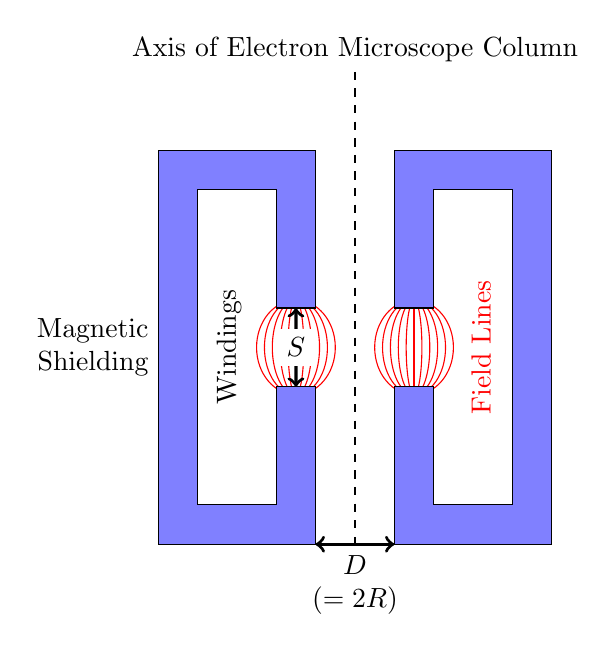
\begin{tikzpicture}
  \foreach \n in {0,0.1,...,0.6}{
    \draw [red] (0.75,-0.5) ellipse [x radius=\n,y radius=0.6];
  }
  \foreach \n in {0,0.1,...,0.6}{
    \draw [red] (-0.75,-0.5) ellipse [x radius=\n,y radius=0.6];
  }
  \draw [fill=blue!50] 
    (-0.5,0)
    -- ++(0,2)
    -- ++(-2,0)
    -- ++(0,-5)
      node [pos=0.5,left,align=right] {Magnetic\\Shielding}
    -- ++(2,0)
    -- ++(0,2)
      coordinate [pos=0] (D left)
    -- ++(-0.5,0)
      coordinate [pos=0.5] (S top)
    -- ++(0,-1.5)
    -- ++(-1,0)
    -- ++(0,4)
    -- ++(1,0)
    -- ++(0,-1.5)
    -- ++(0.5,0)
      coordinate [pos=0.5] (S bottom)
    -- cycle
  ;
  \draw [fill=blue!50] 
    (0.5,0)
    -- ++(0,2)
    -- ++(2,0)
    -- ++(0,-5)
    -- ++(-2,0)
    -- ++(0,2)
      coordinate [pos=0] (D right)
    -- ++(0.5,0)
    -- ++(0,-1.5)
    -- ++(1,0)
    -- ++(0,4)
    -- ++(-1,0)
    -- ++(0,-1.5)
    -- cycle
  ;
  \draw [thick, dashed]
    (0,3)
    -- (0,-3)
      node [pos=0,above] {Axis of Electron Microscope Column}
  ;
  \draw [very thick,<->] 
    (S top) 
    -- (S bottom)
      node [pos=0.5,fill=white] {$S$}
  ;
  \draw [very thick,<->] 
    (D left) 
    -- (D right)
      node [below,pos=0.5,align=center] {$D$\\$(=2R)$}
  ;
  \node [rotate=90] at (-1.6,-0.5) {Windings};
  \node [red,rotate=90] at (1.6,-0.5) {Field Lines};
\end{tikzpicture}

  \caption[Schematic of a generic magnetic lens with a pole-piece]{
    Side-view schematic of a generic magnetic lens with a pole-piece.
    The windings (current loops) are contained within the shielding.
    The magnetic field created by these windings is contained inside the shielding except in the gap.
  }
  \label{fig:polepiece-schematic}
\end{figure}

\begin{figure}
  \centering
  %This work is licensed under the Creative Commons Attribution-NonCommercial-NoDerivs 3.0 United States License. To view a copy of this license, visit http://creativecommons.org/licenses/by-nc-nd/3.0/us/ or send a letter to Creative Commons, 444 Castro Street, Suite 900, Mountain View, California, 94041, USA.

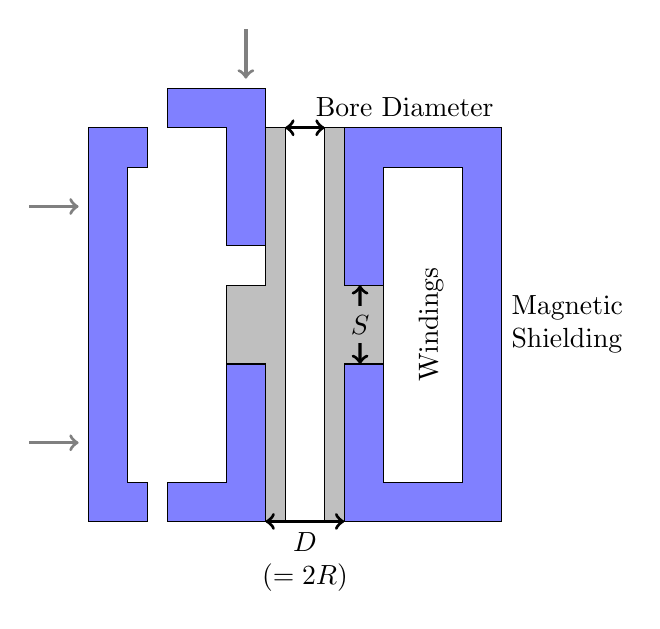
\begin{tikzpicture}
  \draw [fill=blue!50] 
    (-0.5,0.5)
    -- ++(0,2)
    -- ++(-1.25,0)
      node [pos=0.2] (assemble top) {}
    -- ++(0,-0.5)
    -- ++(0.75,0)
    -- ++(0,-1.5)
    -- ++(0.5,0)
    -- cycle
  ;

  \draw [very thick, <-, gray]
    (assemble top)
    -- ++(0,0.75)
  ;

  \draw [fill=blue!50]
    (-2,2)
    -- ++(-0.75,0)
    -- ++(0,-5)
      node [pos=0.2] (assemble left upper) {}
      node [pos=0.8] (assemble left lower) {}
    -- ++(0.75,0)
    -- ++(0,0.5)
    -- ++(-0.25,0)
    -- ++(0,4)
    -- ++(0.25,0)
    -- cycle
  ;

  \draw [very thick, <-, gray]
    (assemble left upper)
    -- ++(-0.75,0)
  ;
  \draw [very thick, <-, gray]
    (assemble left lower)
    -- ++(-0.75,0)
  ;

  \draw [fill=blue!50] 
    (-0.5,-1)
    -- ++(0,-2)
      coordinate [pos=1] (D left)
    -- ++(-1.25,0)
    -- ++(0,0.5)
    -- ++(0.75,0)
    -- ++(0,1.5)
    -- ++(0.5,0)
    -- cycle
  ;

  \draw [fill=blue!50] 
    (0.5,0)
    -- ++(0,2)
    -- ++(2,0)
    -- ++(0,-5)
      node [pos=0.5,right,align=left] {Magnetic\\Shielding}
    -- ++(-2,0)
    -- ++(0,2)
      coordinate [pos=0] (D right)
    -- ++(0.5,0)
    -- ++(0,-1.5)
    -- ++(1,0)
    -- ++(0,4)
    -- ++(-1,0)
    -- ++(0,-1.5)
    -- ++(-0.5,0)
    -- cycle
  ;

  \draw [fill=gray!50]
    (-0.5,2)
    -- ++(-0,-2)
    -- ++(-0.5,0)
    -- ++(0,-1)
    -- ++(0.5,0)
    -- ++(0,-2)
    -- ++(0.25,0)
    -- ++(0,5)
      coordinate [pos=1] (B left)
    -- ++(-0.25,0)
    -- cycle
  ;

  \draw [fill=gray!50]
    (0.5,2)
    -- ++(-0,-2)
    -- ++(0.5,0)
      coordinate [pos=0.4] (S top)
    -- ++(0,-1)
    -- ++(-0.5,0)
      coordinate [pos=0.6] (S bottom)
    -- ++(0,-2)
    -- ++(-0.25,0)
    -- ++(0,5)
      coordinate [pos=1] (B right)
    -- ++(0.25,0)
    -- cycle
  ;

  \draw [very thick,<->] 
    (S top) 
    -- (S bottom)
      node [pos=0.5,fill=gray!50] {$S$}
  ;
  \draw [very thick,<->] 
    (D left) 
    -- (D right)
      node [below,pos=0.5,align=center] {$D$\\$(=2R)$}
  ;
  \draw [very thick,<->] 
    (B left) 
    -- (B right)
      node [above right,pos=0.5,align=center] {Bore Diameter}
  ;
  \node [rotate=90] at (1.6,-0.5) {Windings};
\end{tikzpicture}

  \caption[Design schematic of our magnetic lens with a pole-piece]{
    Side-view schematic of the magnetic lens with a pole-piece designed for the UEM at UIC.
    On the center axis is the inner drift tube, with pole-piece gap separation disk.
    The end pieces are shown top and bottom, bridges are on the left and right.
    The left side shows a bridge piece and one end before assembly.
    Note that this figure is not drawn to the scale of the lenses at UIC, but rather to match the general schematic in \ref{fig:polepiece-schematic}.
  }
  \label{fig:polepiece-design}
\end{figure}

\ref{fig:polepiece-design} shows a schematic of the lens designed and built for the UEM at UIC.
The central drift tube is made of stainless steel having a magnetic permeability of 1, thus magnetically not involved in the field shaping.
In this way only the inner bore of the tube may be in vacuum thus minimizing necessary welding.
The outer diameter of tube is machined down to $ D = 2R = 0.5 \text{in}$, though a disk of larger diameter, and length $ S = $ 0.1in, is left at the midpoint, which will separate the shielding material and be the pole-piece gap.

The high magnetic permeability shielding is made of eleven pieces.
There are two end pieces which are revolution solids of an ``L'' shaped profile.
These ends slide together over the drift tube until touching the disk at the midpoint; the disk is of the proper outer diameter to match the sheilding's smaller outer diameter.
The combination of the two ends and this disk make a ``U'' shape which contains the windings.
The top of the each end's large outer disk (the walls of the winding container) are flattend on eight sides.
These are the mount points for eight bridge pieces which connect the ends to complete the field-capturing shielding loop.
The gaps between the shielding bridges also allow for direct air cooling of the magnetic coils (see Section \ref{sec:mag_lens_thermal}).

El-Kareh and El-Kareh provide an analysis for symmetric lenses with magnetic shielding and a pole-piece (see Ref. \cite{el-kareh_electron_1970} chapter 8, with the most useful information being in section 8.7).
They define two parameters,
\begin{equation}
  k^2 \equiv \frac{e}{8 m V_r} B_0^2 R^2
\end{equation}
and
\begin{equation} \label{eq:elkareh_k2}
  \beta \equiv k^2 V_r / (NI)^2 \,\text{,}
\end{equation}
where $N$ is the number of loops, $I$ is the current in a single loop, $B_0$ is the maximum axial magnetic field strength, $R$ is the bore radius and $V_r$ is the relativity corrected acceleration potential, given by
\begin{equation}
  V_r = V ( 1 + \frac{0.978 \cdot 10^{-6}}{\text{Volt}} V ) \,\text{.}
\end{equation}
Using the provided tabulated results, and for a choice of parameters one can determine the number of ampere-turns ($NI$) to create a certain focal length.
Since the drift tube has an outer diameter $D=$0.5in and the pole-piece gap length is $S$=0.1in, the lens has a ratio $S/D=0.2$.
By their table 8.2a this results in $\beta=0.0146$.
Then, to create a focal length of 4in ($f/R=16$) table 8.13 in Ref. \cite{el-kareh_electron_1970} gives a value for $k^2 \approx 0.06$.
Finally substituting this value into \ref{eq:elkareh_k2}, with $V=30$kV ($V_r\approx30.88$kV), one can deduce that $NI\approx356$A.

For the UEM system at UIC, two of these lenses are employed to manage the divergence created by an RF cavity and the anode aperture, then focus the pulses to a focal spot. 
These lenses are positioned one before and one after the RF cavity, forming a lens system of a combined effective focal length; the two lenses are wound oppositely to counteract beam rotation.
For the purposes of design, one can make a reasonable approximation that the two lenses together provide the total necessary number of amp-turns.
As each lens has 100 turns, a current of only about 2A is needed to drive the two lenses in series to attain a 4in focal length.
A picture of this system is shown in \ref{fig:maglens-pic}.
In that picture the two lenses are shown, however a placeholder is shown inserted between them rather than an actual RF cavity.

\begin{figure}
  \centering
  \includegraphics{maglens.jpg}
  \caption[Side-view picture of the employed two custom large-bore magnetic lenses]{
    Side-view of the two custom large-bore magnetic lenses designed and built at UIC, seen installed in the prototype UEM.
    The coils are visible in the gaps between the high permeability shielding ``bridges''.
    The bridges are attached to the tops of the end pieces by bolts to complete the shielding loop.
    The outer (larger) plates and struts are for structural integrity only.
  }
  \label{fig:maglens-pic}
\end{figure}

\subsection{Thermal Properties} \label{sec:mag_lens_thermal}

%TODO need reference for equation and \alpha_{Cu}
As the lenses have no active cooling system, it was prudent to characterize the thermal response to a moderate current load.
Resistance of metals changes as a function of temperature by $ R = R_0 [ 1 + \alpha ( T - T_0 ) ] $, where $\alpha$ is a material contant; for copper, $\alpha = 3.9 * 10^{-3} \text{K}^{-1}$. 
One can calculate the temperature increase of the system by monitoring the change in resistance.
Maintaining a constant current of 4A through the lens, the voltage drop increased from 1.22V ($R_0 = 0.305\Omega$) to 1.25V ($R=0.3125\Omega$) as the lens warmed.
The resultant temperature increase is only $T - T_0 = 2\text{K}$.
This result is easily confirmed manually; the oxygen-free copper wire coils remain cool to the touch under these operating conditions.

